%\documentclass[border=10pt]{standalone}
%\usepackage{tikz}
\tikzset{
	treenode/.style = {shape=rectangle, rounded corners,
		draw, align=center,
		top color=white, bottom color=blue!20},
	root/.style     = {treenode, font=\ttfamily\normalsize, bottom color=red!30},
	env/.style      = {treenode, font=\ttfamily\normalsize},
	dummy/.style    = {circle,draw},
	level 1/.style={sibling distance=6cm, level distance = 3em},
	level 2/.style={sibling distance=2.5cm,level distance = 5em}, 
	level 3/.style={sibling distance=2cm},
	blueRed/.style={env, top color=blue, bottom color=red} 
}
%\begin{document}
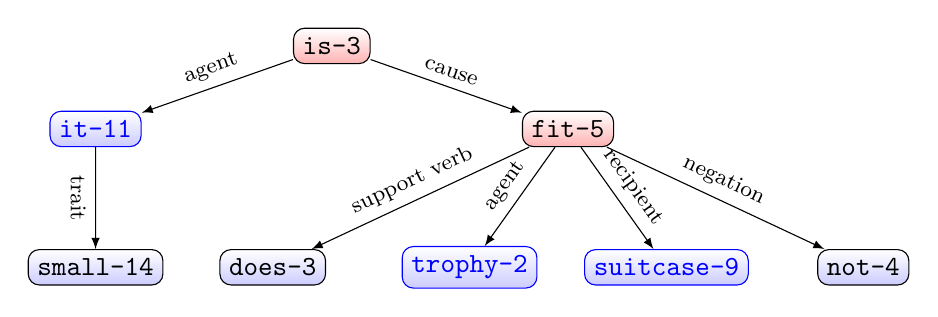
\begin{tikzpicture}
[
grow                    = down,
sibling distance        = 50em,
level distance          = 5em,
edge from parent/.style = {draw, -latex},
every node/.style       = {font=\footnotesize},
sloped
]
\node [root] {is-3}
child { node [env, blue] {it-11}
	child {node [env] {small-14}
		edge from parent node [below] {trait} }
	edge from parent node [above] {agent}}
child { node [env, bottom color=red!30] {fit-5} 
	child {node [env]  {does-3}
		edge from parent node [above] {support verb} }	
	child {node [env, blue]  {trophy-2}
		edge from parent node [above] {agent} }
	child {node [env, blue]  {suitcase-9}
		edge from parent node [above] {recipient}}
	child {node [env]  {not-4}
		edge from parent node [above] {negation} }
	edge from parent node [above] {cause}};

\end{tikzpicture}
%\end{document}